\subsection{Hidden Markov Models}
\label{subsec:ch4sec1subsec1}

A Markov Model provides a probabilistic representation 
of relationship between a given set of events under the premise that the future evolution of the system only depends on the current state and not on the previous ones \cite{Jurafsky}. It can be mathematically described as a graph $(Q,A)$, where the nodes $q_i \in Q$ denote the states and the edges $a_{ij}\in A$ hold the probability of transitioning from the state $q_{i}$ to a state ${q_j}$. Each node is assigned an initial probability $\pi_i$ determining whether the model is more or less likely to start from node $q_i$. Sometimes, some events are not directly readable and their nature must be deduced from the known observations, in which case they are called hidden events. A Hidden Markov Model (HMM) specializes in handling a sequence of observations $O=o_1\ldots o_T$ and for each node ${q_i}$ compute an observation likelihood $b_i(o_t)\in B$ at each timestamp $t=1\ldots T$ \cite{Jurafsky}. The sets $A$ and $B$ of probabilities provide a propitious playground for training methods, such as the forward-backward algorithm \cite{Jurafsky}. The HMM also needs a decoder to find the most probable sequence of states $q_{i_1}\ldots q_{i_x}$ starting from a given set of observations $o_1\ldots o_T$. We remind the Viterbi algorithm as an example of such decoder \cite{Jurafsky}.

\begin{figure}[htbp]
	\centering
		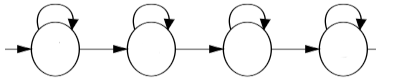
\includegraphics[scale=1]{figures/hmm_lin}
	\caption{HMM linear topology \cite{hmm_linear_model}}
	\label{FigHMMLinear}        
\end{figure}


HMM has seen successful applications in speech recognition and online HTR problems \cite{Juan}, although it can be applied to some extend to offline cursive text recognition \cite{HMM_dict}. HMMs can work at char level, such as a 6 states left-to-right model \cite{HMM_char}, or at word level, by creating small sized dictionaries of words that the model can predict \cite{HMM_dict}. Hidden Markov Models have a long history in character recognition \cite{HmmSurvey}. However, their performance becomes obsolete as they are eclipsed by the advancement of the more powerful deep learning models \cite{cnnbilstm}.

\subsection{CNN-RNN Networks}
\label{subsec:ch4sec1subsec2}

The effectiveness of CNNs in features extraction makes it a favorable starting point when it comes to working with images. This way, an image can be encoded into a sequence of features that is conveniently passed to a recurrent network for analysis. This formula has been proven to outperform previous models like the RNN-only, which is suitable for individual characters recognition, ensuring prior segmentation, or the hybrid CNN-HMM or HMM-RNN models \cite{Juan}. 

The CNN-RNN model takes advantage of both the image featues and the sequenciality of the data, this becoming the state of the art in the HTR problem \cite{Juan}. Furthermore, in order to deal with non-uniformities regarding features dilations over timestamps (e.g. a handwritten "m" is taking more space than a "t" letter), researchers have passed the output of the RNN to a CTC decoder that help link adjacent timestamps to the a single observation when needed \cite{cnnrnn}. 

The prediction is also paired with the labeled output from the dataset in order to produce a CTC loss that will be used to train the model \cite{cnnrnn}. For an improved clarity, the author of the current thesis has visibly separated the concepts of training and decoding, as shown in figure \ref{FigCNNRNN}. This way, the CTC layer would not manifest different behaviors at training and prediction time. Moreover, the ground truth data is not needed (neither is accessible) outside the training process.

\begin{figure}[htbp]
	\centering
		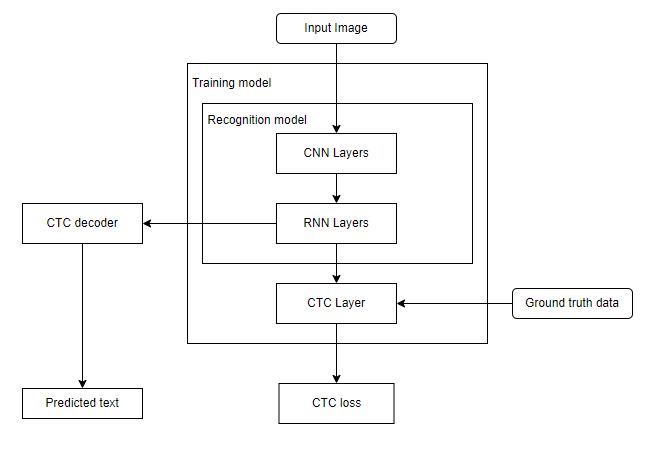
\includegraphics[scale=0.75]{figures/cnn_rnn_model}
	\caption{General CNN-RNN model flowchart}
	\label{FigCNNRNN}        
\end{figure}

The usage of a bidirectional LSTM as the underlaying recurrent network seems to stands out in front of other RNN architectures \cite{cnnbilstm}. However, they also have their limitations imposed by the overall structure itself. The CNN-RNN model performs great on predicting lines of text, but may struggle with processing whole paragraphs. Moreover, increasing the number of RNN timestamps comes at the cost of decreased performance \cite{Juan}. Training a CTC model is tedious as the model starts by only predicting blank labels in its first epochs. Theodore Bluche has an insighful research regarding the CTC performance and the optimal choice for the number of timestamps \cite{TBluche}.

\subsection{Multi-Dimensional LSTM}
\label{subsec:ch4sec1subsec3}

The idea of introducing a multi- (in this case, two-) dimensional RNN solution to the HTR problem seems quite natural since we are working with bidimensional data \cite{Juan}. The main promise of MDLSTM over the traditional sequence-to-sequence RNN models is the ability to perform full-page text recognition with minimum or no amount of preprocessing and segmentation \cite{MDLSTM}. 

\begin{figure}[htbp]
	\centering
        \begin{floatrow}
             \ffigbox{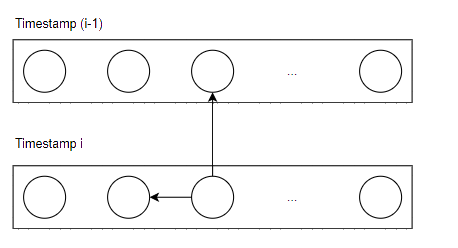
\includegraphics[scale = 0.6]{figures/rnn_fw}}{\caption{1D RNN forward pass}\label{fig1drnn}}             
             \ffigbox{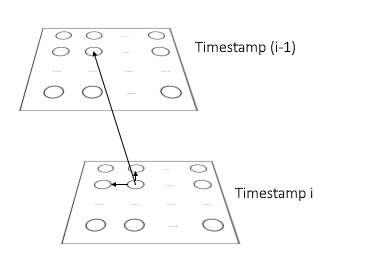
\includegraphics[scale = 0.7]{figures/rnn2d_fw}}{\caption{2D RNN forward pass}\label{fig2drnn}}
        \end{floatrow}                 
\end{figure}

When computing a hidden state $h_{i,j}^t$ at timestamp $t$, a 2D RNN accounts for the input $x_{i,j}^{t}$, as well as the adjacent states at current timestamp, $h_{i-1,j}^t$, $h_{i,j-1}^t$ \cite{mdrnn} as seen in figure \ref{fig2drnn}.

Following the fact that "we can easily this [the one dimensional LSTM implementation - Ed.] to $n$ dimensions"\cite{mdrnn}, the author has attempted to implement their own version of a MDLSTM cell for the particular case $n=2$, motivated by the lack of built-in support for MDLSTM in the used machine learning framework. The flow graph diagram is showcased in figure \ref{FigMDLSTM}. The hidden state and cell memory inputs, plus the forget gate, have duplicate correspondents, one for each dimension, as the source indicates \cite{mdrnn}. Consequently, the individual computations for each dimensions are being wired together by addition operations leading to the cell's output. 


\begin{figure}[htbp]
	\centering
		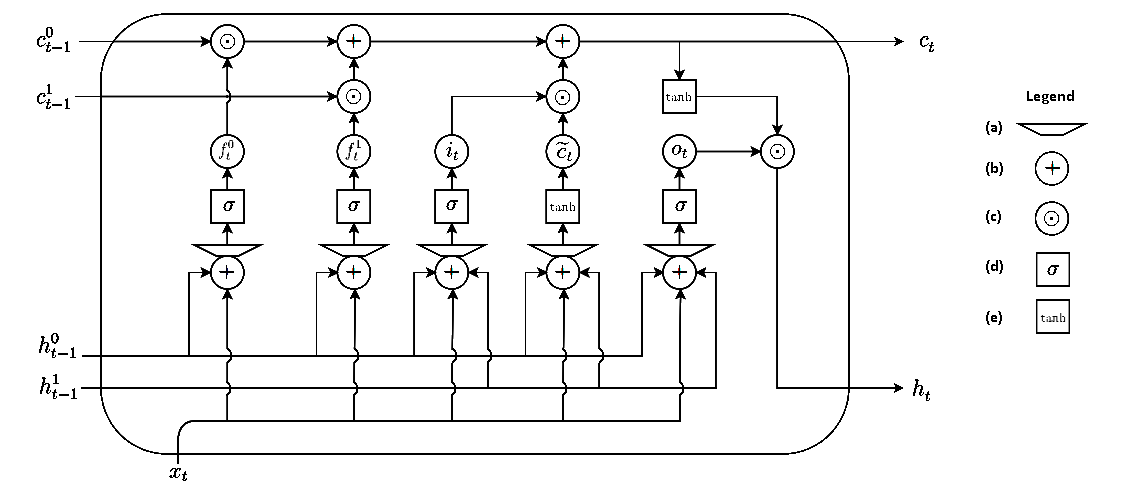
\includegraphics[scale=0.5]{figures/mdlstm_cell}
	\caption{\centering 2-dimensional MDLSTM cell. \newline Legend: \textit{(a) dense layer; (b) addition; (c) Hadamard product; (d) sigmoid activation; (e) tanh activation.}}
	\label{FigMDLSTM}        
\end{figure}

The multidimensional character of such a layer justifies its place in a network right after a (possibly filtered) image. Graves et. al, who introduced this aproach in HTR problems, use multiple stacked MDLSTM layers working on a tiled image to achieve words recognition. They keep increasing the cells count with each layer while halfing the input shape in a similar way one would craft a CNN-based model \cite{GravesMDLSTM}.    Bluche  et al. take it one step further and infer convolution layers between MDLSTMs \cite{MDLSTM}. The CNNs organize and enhance the feature extraction, while the recurrent layers are also responsible for downsampling the data. Furthermore, it is not uncommon to also extend the bidirectional RNN approach to a multidirectional MDRNN/MDLSTM. The idea is to traverse the input forward and backward on each of the $n$ dimensions with a separate multidimensional layer. The $2^n$ results obtained from those layers are then accumulated, either by some element-wise aggregation or concatenation into a single output \cite{mdrnn}. We can immediately observe that this approach quickly becomes infeasible when a higher dimensions count $n$ is concerned.

Author's experiments have confirmed that MDLSTMs are computationally slow in a way that undermines their advantage in exploiting data dimensionality, as literature sources state \cite{MDLSTM_analysis} \cite{Juan}. As in the usual case of RNN architectures, the dependence of one state on the previous ones makes parallelization difficult, and some GPU optimizing techniques like loop unrolling are resource intensive and can only be applied on small quantities of data.

\subsection{Transformer models}
\label{subsec:ch4sec1subsec4}

The transformer model is a relatively recent product in the science of deep learning. They came into light in 2017 and have quickly grown in popularity due to their applications and proven effectiveness in a wide area of fields, from language translation to image processing \cite{Juan}. They provide an alternative solution to seq2seq problems inspired by mimicking the way biological creature interact and learn the environment through the attention mechanism. They are lightweight, highly parallelizable are perform better at handling long-range dependencies, but their require larger training datasets \cite{transformerNlp}.

\begin{figure}[htbp]
	\centering
		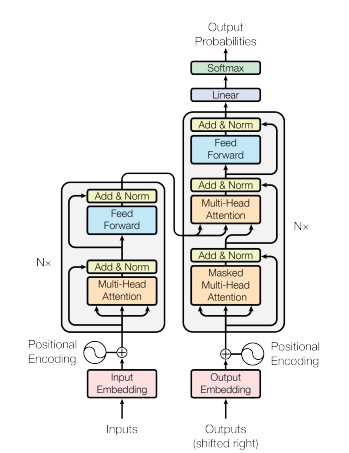
\includegraphics[scale=0.7]{figures/transformer}
	\caption{Transformer architecture \cite{transformer}}
	\label{FigTransformer}        
\end{figure}

A transformer consists of two main components as shown in figure \ref{FigTransformer}: an encoder and a decoder \cite{transformer}. A positional embedding is applied to each sample of input to engrave a sense of sequentiality into it, in order to cope with the fact that the architecture does not account for order. This is done usually by adding to the sample a sine wave of a frequency chosen in a clever way that allows for identifying the original position of a certain piece of data in the original sequence \cite{transformer}. The encoder consists of multiple stacked blocks that contain a multi-head attention layer and a dense (feed forward) layer. Thus, it produces an encoded $d$-dimensional vector for each sample at a given position \cite{D2l}. The decoder borrows the previous block structure, with a new multi-head attention inserted between the two layers, called encoder-decoder attention, whose role is to build a bridge between the two transformer components. The encoder's outputs become keys and values in the attention layer, while the decoder provides the queries \cite{D2l}. The decoder's masked attention ensures that the attention only considers data up to a certain position, so that a prediction is made only in function of already generated samples \cite{D2l}. Furthermore, a version of this architecture was designed to be suitable for image processing, giving birth to the Visual Transformer (ViT), which deals with sequences of equally sized partitions from the input image, helping it efficiently combine local information with global self-attention \cite{vit}. MSdocTr-Lite is an example of the application of a transformer in the field of handwritten text recognition \cite{msdoctrlite}.